\section*{Question 1.1}

The following plot has been produced through straightforward use of
the \texttt{dnorm} function and plotting facilities in R.  A thousand
sample points have been used.  The code for this question is in the
file \texttt{question11.R}.

\begin{figure}
 \begin{centering}
    % GNUPLOT: LaTeX picture with Postscript
\begingroup
  \makeatletter
  \providecommand\color[2][]{%
    \GenericError{(gnuplot) \space\space\space\@spaces}{%
      Package color not loaded in conjunction with
      terminal option `colourtext'%
    }{See the gnuplot documentation for explanation.%
    }{Either use 'blacktext' in gnuplot or load the package
      color.sty in LaTeX.}%
    \renewcommand\color[2][]{}%
  }%
  \providecommand\includegraphics[2][]{%
    \GenericError{(gnuplot) \space\space\space\@spaces}{%
      Package graphicx or graphics not loaded%
    }{See the gnuplot documentation for explanation.%
    }{The gnuplot epslatex terminal needs graphicx.sty or graphics.sty.}%
    \renewcommand\includegraphics[2][]{}%
  }%
  \providecommand\rotatebox[2]{#2}%
  \@ifundefined{ifGPcolor}{%
    \newif\ifGPcolor
    \GPcolortrue
  }{}%
  \@ifundefined{ifGPblacktext}{%
    \newif\ifGPblacktext
    \GPblacktextfalse
  }{}%
  % define a \g@addto@macro without @ in the name:
  \let\gplgaddtomacro\g@addto@macro
  % define empty templates for all commands taking text:
  \gdef\gplbacktext{}%
  \gdef\gplfronttext{}%
  \makeatother
  \ifGPblacktext
    % no textcolor at all
    \def\colorrgb#1{}%
    \def\colorgray#1{}%
  \else
    % gray or color?
    \ifGPcolor
      \def\colorrgb#1{\color[rgb]{#1}}%
      \def\colorgray#1{\color[gray]{#1}}%
      \expandafter\def\csname LTw\endcsname{\color{white}}%
      \expandafter\def\csname LTb\endcsname{\color{black}}%
      \expandafter\def\csname LTa\endcsname{\color{black}}%
      \expandafter\def\csname LT0\endcsname{\color[rgb]{1,0,0}}%
      \expandafter\def\csname LT1\endcsname{\color[rgb]{0,1,0}}%
      \expandafter\def\csname LT2\endcsname{\color[rgb]{0,0,1}}%
      \expandafter\def\csname LT3\endcsname{\color[rgb]{1,0,1}}%
      \expandafter\def\csname LT4\endcsname{\color[rgb]{0,1,1}}%
      \expandafter\def\csname LT5\endcsname{\color[rgb]{1,1,0}}%
      \expandafter\def\csname LT6\endcsname{\color[rgb]{0,0,0}}%
      \expandafter\def\csname LT7\endcsname{\color[rgb]{1,0.3,0}}%
      \expandafter\def\csname LT8\endcsname{\color[rgb]{0.5,0.5,0.5}}%
    \else
      % gray
      \def\colorrgb#1{\color{black}}%
      \def\colorgray#1{\color[gray]{#1}}%
      \expandafter\def\csname LTw\endcsname{\color{white}}%
      \expandafter\def\csname LTb\endcsname{\color{black}}%
      \expandafter\def\csname LTa\endcsname{\color{black}}%
      \expandafter\def\csname LT0\endcsname{\color{black}}%
      \expandafter\def\csname LT1\endcsname{\color{black}}%
      \expandafter\def\csname LT2\endcsname{\color{black}}%
      \expandafter\def\csname LT3\endcsname{\color{black}}%
      \expandafter\def\csname LT4\endcsname{\color{black}}%
      \expandafter\def\csname LT5\endcsname{\color{black}}%
      \expandafter\def\csname LT6\endcsname{\color{black}}%
      \expandafter\def\csname LT7\endcsname{\color{black}}%
      \expandafter\def\csname LT8\endcsname{\color{black}}%
    \fi
  \fi
  \setlength{\unitlength}{0.0500bp}%
  \begin{picture}(7200.00,5040.00)%
    \gplgaddtomacro\gplbacktext{%
      \csname LTb\endcsname%
      \put(1078,704){\makebox(0,0)[r]{\strut{} 0}}%
      \put(1078,1168){\makebox(0,0)[r]{\strut{} 0.05}}%
      \put(1078,1632){\makebox(0,0)[r]{\strut{} 0.1}}%
      \put(1078,2096){\makebox(0,0)[r]{\strut{} 0.15}}%
      \put(1078,2559){\makebox(0,0)[r]{\strut{} 0.2}}%
      \put(1078,3023){\makebox(0,0)[r]{\strut{} 0.25}}%
      \put(1078,3487){\makebox(0,0)[r]{\strut{} 0.3}}%
      \put(1078,3951){\makebox(0,0)[r]{\strut{} 0.35}}%
      \put(1078,4415){\makebox(0,0)[r]{\strut{} 0.4}}%
      \put(2089,484){\makebox(0,0){\strut{}-5}}%
      \put(3246,484){\makebox(0,0){\strut{} 0}}%
      \put(4402,484){\makebox(0,0){\strut{} 5}}%
      \put(5559,484){\makebox(0,0){\strut{} 10}}%
      \put(6715,484){\makebox(0,0){\strut{} 15}}%
      \put(176,2739){\rotatebox{-270}{\makebox(0,0){\strut{}Y}}}%
      \put(4006,154){\makebox(0,0){\strut{}X}}%
    }%
    \gplgaddtomacro\gplfronttext{%
      \csname LTb\endcsname%
      \put(5816,4602){\makebox(0,0)[r]{\strut{}$\mu$=-1, $\sigma$=1}}%
      \csname LTb\endcsname%
      \put(5816,4382){\makebox(0,0)[r]{\strut{}$\mu$=2, $\sigma$=2}}%
      \csname LTb\endcsname%
      \put(5816,4162){\makebox(0,0)[r]{\strut{}$\mu$=3, $\sigma$=3}}%
    }%
    \gplbacktext
    \put(0,0){\includegraphics{tex_out/case1}}%
    \gplfronttext
  \end{picture}%
\endgroup

%  \label{foobar}
 \end{centering}
\end{figure}


\section*{Question 1.2}

The matrix
\[
M=\left[\begin{matrix}
  x_{1,1}&\cdots&x_{1,m}\\\vdots&\ddots&\vdots\\x_{n,1}&\cdots&x_{n,m} \end{matrix}\right]
\]
is \textit{positive definite} if for any nonzero real-entried vector
\[
V=\left[\begin{matrix} y_1 \\ \vdots \\ y_m \end{matrix}\right]
\]
we have
\[
V^TMV > 0.
\]

$M$ is \textit{symmetric} if $M^T=M$.

$M$ is \textit{square} if $m=n$.

An eigenvalue $\lambda$ is positive if $\lambda > 0$.

\section*{Question 1.3}

The code for this question is in the file \texttt{question131415.R}.

\includegraphics[width=10cm]{img/question13-plot.eps}

\section*{Question 1.4}

The code for this question is in the file \texttt{question131415.R}

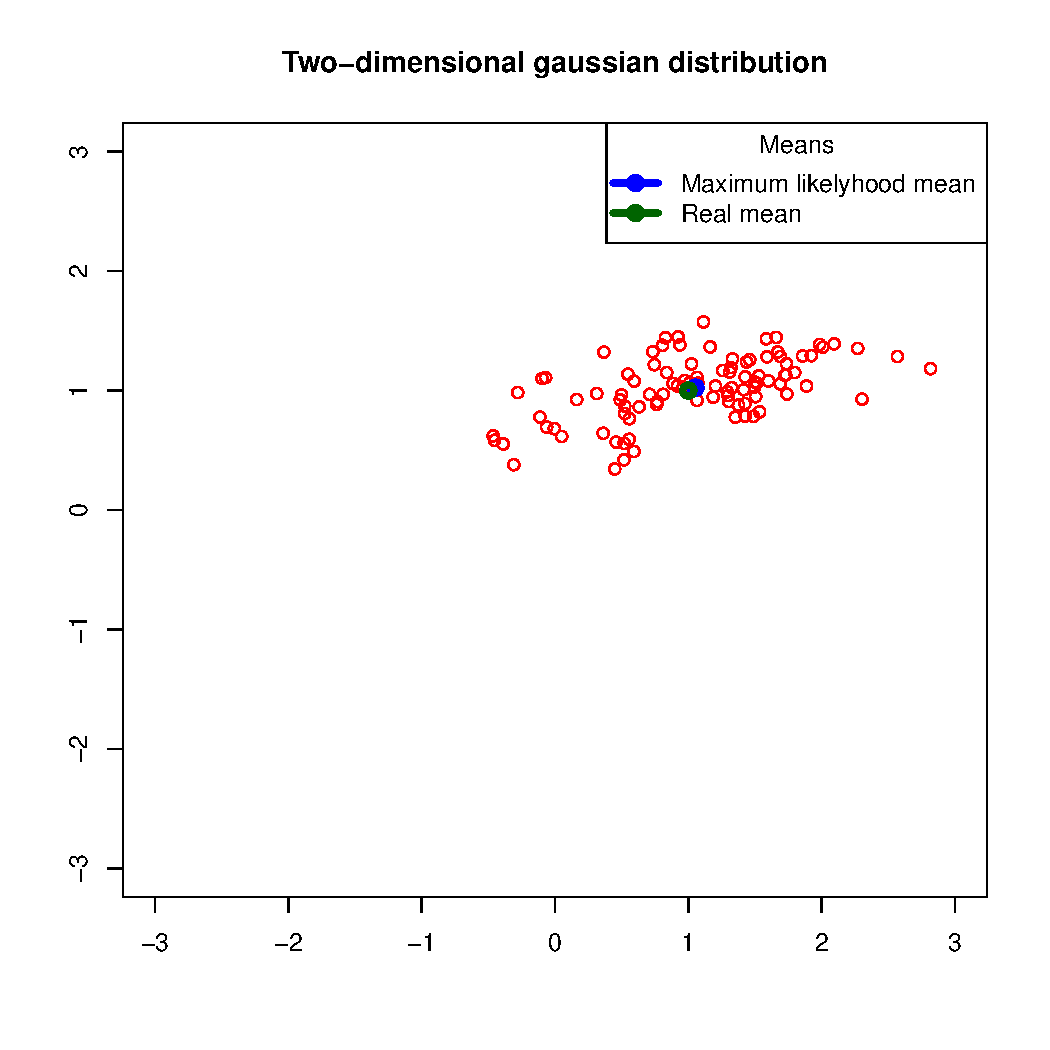
\includegraphics[width=10cm]{img/question14-plot.eps}

On a particular sampling the following sample covariance was observed
\[
\left[\begin{matrix}0.3085769&0.2101958\\0.2101958&0.2042408\end{matrix}\right]
\]
along with the sample mean
\[
\left[\begin{matrix}0.9855921\\0.9914642\end{matrix}\right]
\]

The Euclidian distance from the sample mean to the real mean is
\[
\sqrt{(0.9855921-1)^2+(0.9914642-1)^2}=0.01674
\]

This deviation could be due to the low number of samples.

\section*{Question 1.5}

The code for this question is in the file \texttt{question131415.R}.\\
\includegraphics{img/question15-plot-1-a.eps}
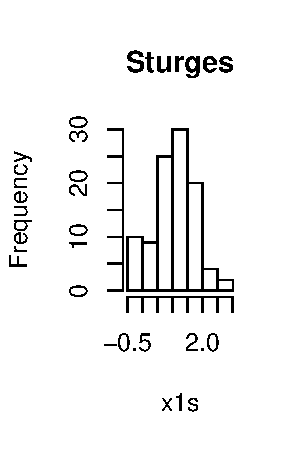
\includegraphics{img/question15-plot-1-b.eps}
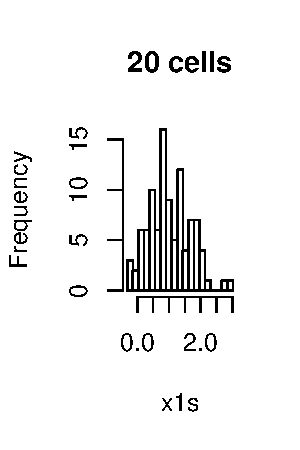
\includegraphics{img/question15-plot-1-c.eps}
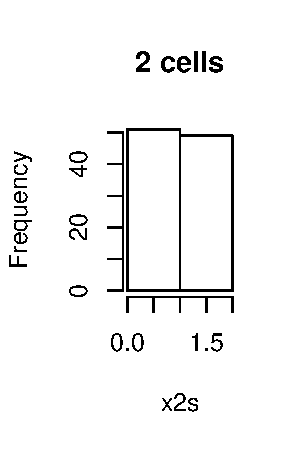
\includegraphics{img/question15-plot-2-a.eps}
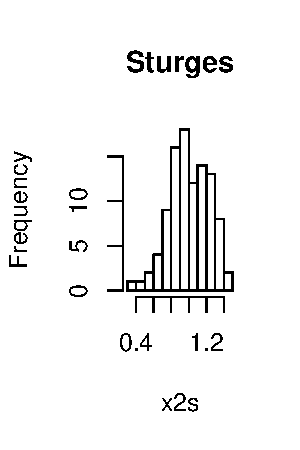
\includegraphics{img/question15-plot-2-b.eps}
\includegraphics{img/question15-plot-2-c.eps}

As the bin width decreases, the random variation in the data results
in new local maximums that make the distribution appear more jagged
than it really is.

There is no best method to select bin widths, as the.  A common
method is Sturges' formula, where the $n$ data points are divided into
$\lceil\log_2n+1 \rceil$ bins.

\section*{Question 1.6}

The histogram is plotted with respect to density, rather than
frequency, so it can be easily compared to the density curve.  As can
be seen, the histogram with six bars fits the analytical curve well.

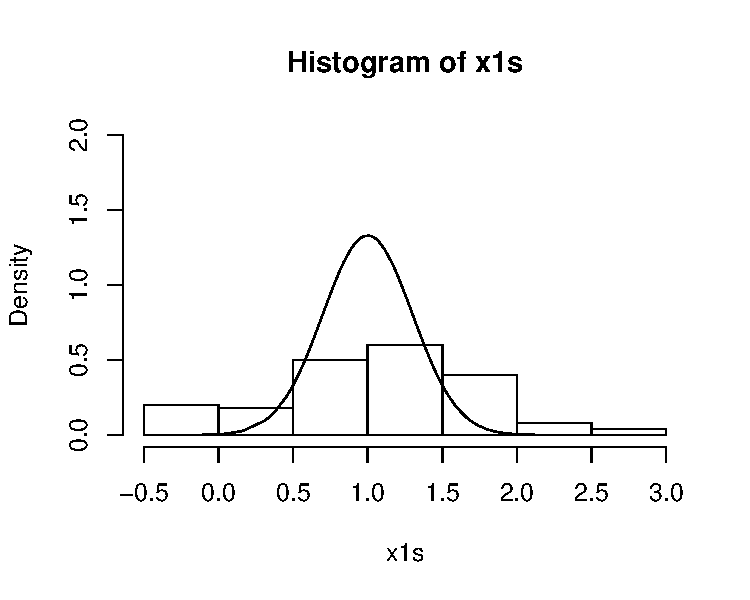
\includegraphics{img/question16-plot-analytical.eps}

The marginal distribution has the following analytical expression.

\begin{align*}
  p(x_1) &= \mathcal{N}(x_1|\mu_1,\Sigma_{1,1}) & \text{By CB (2.98)}\\
  &=
  \frac{1}{(2\pi\sigma_{1,1}^2)^{1/2}}\exp\left({-\frac{1}{2\sigma_{1,1}^2}(x_1-\mu_1)^2}\right)
  & \text{Substituting definition} \\
  &=
  \frac{1}{(2\pi\cdot 0.2^2)^{1/2}}\exp\left({-\frac{1}{2\cdot0.2^2}(x_1-1)^2}\right)
  & \text{Substituting $\sigma_{1,1}=0.2,\mu_1=1$}
\end{align*}

\section*{Question 1.7}

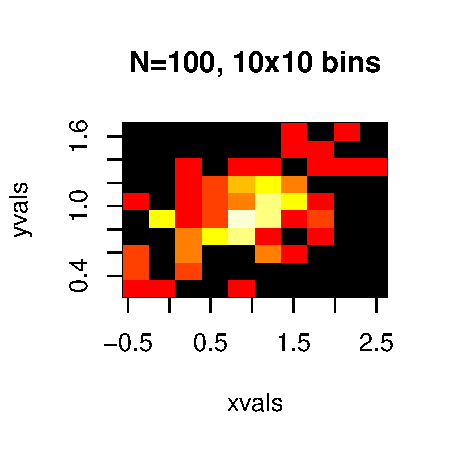
\includegraphics{img/question17-plot-100.eps}
\includegraphics{img/question17-plot-1000-10x10.eps}
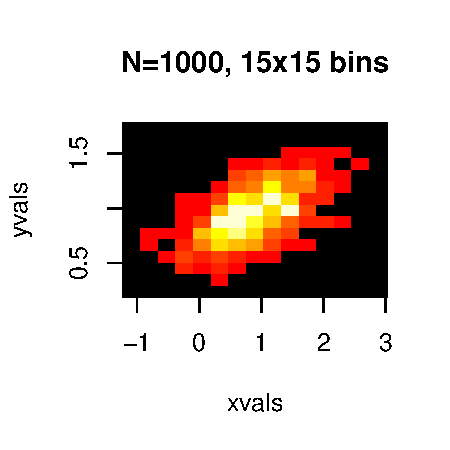
\includegraphics{img/question17-plot-1000-15x15.eps}
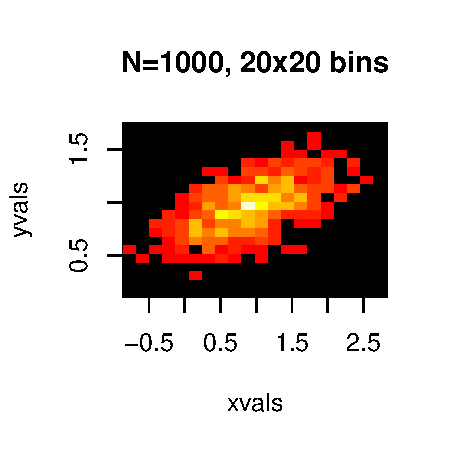
\includegraphics{img/question17-plot-1000-20x20.eps}
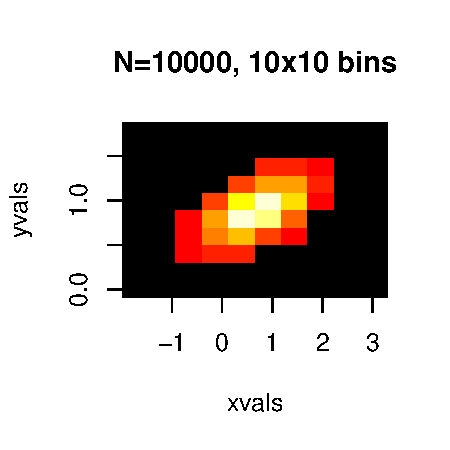
\includegraphics{img/question17-plot-10000.eps}

\section*{Question 1.8}


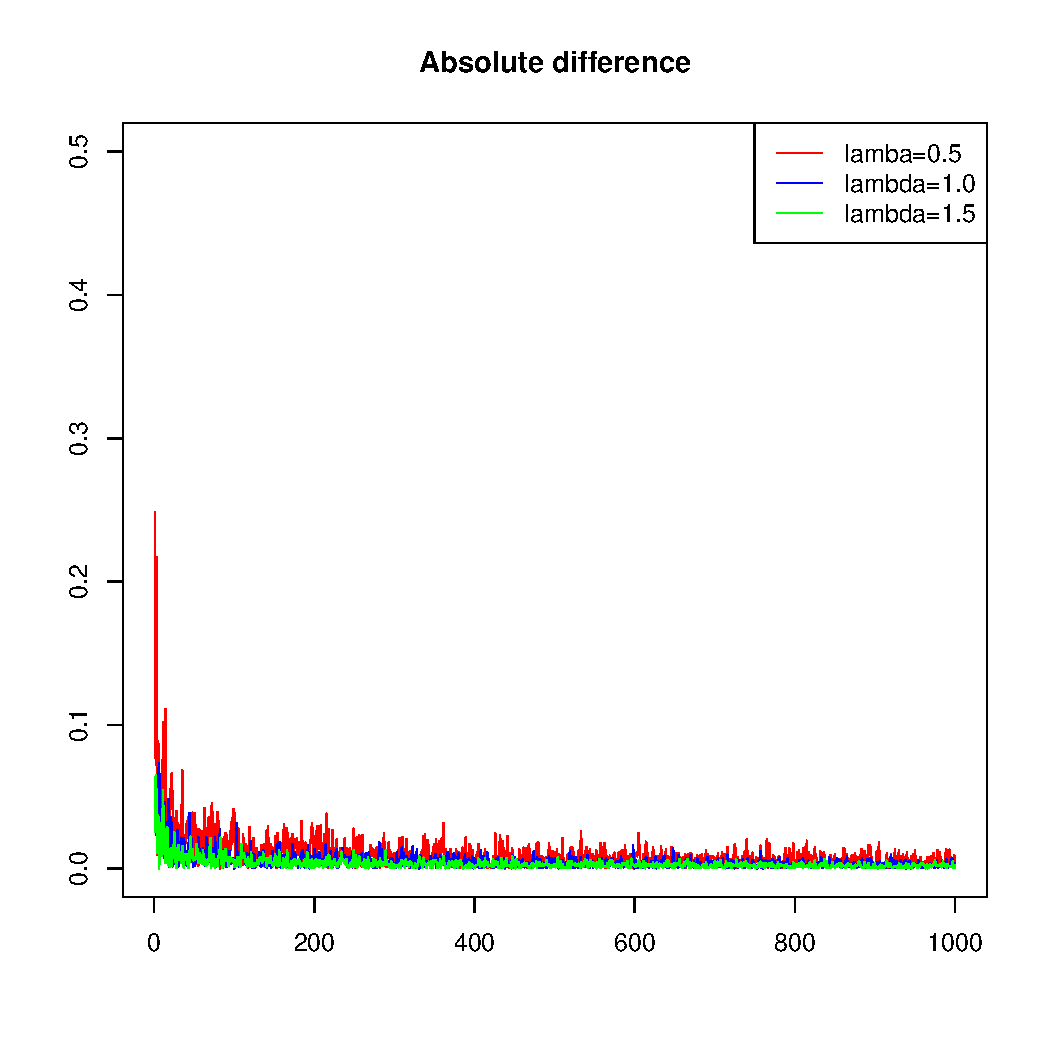
\includegraphics[width=10cm]{img/question18-plot-1.eps}

On a logarithmic $y$-axis, the plot above would consist of straight
lines.
